\chapter{One-dimensional finite-volume methods}
\label{chp1-1d-fv}
The main aim of this chapter is to give a detailed desctription of
the Piecewise Parabolic Method (PPM).
We start with a basic review on one-dimensional conservation laws in
the integral form in Section \ref{chp1-sec1}, 
and in Section \ref{chp1-sec2} we set the framework of
general one-dimensional finite-volumes schemes.
Section \ref{chp1-sec-ppm} presents and analyses the PPM in Subsection \ref{chp1-sec-recon}.
Subsection \ref{chp1-sec-mono} is dedicated to PPM monotonization
and Subsection \ref{chp1-sec-flux} is dedicated to the PPM flux.
At last, Section \ref{chp1-sec-numerical-exp} shows some numerical results using the PPM scheme.

\section{One-dimensional system of conservation laws in integral form}
\label{chp1-sec1}
In this section, we are going to present the derivation of one-dimensional 
system of conservation laws in the integral form. 
The derivation presented here follows \citet{leveque:1990} and \citet{leveque:2002} closely and will
be useful to fix some notation. \index{Conservation law}
Let us assume that $x$ and $t$ represent the spatial and time coordinate, respectively.
Given $[x_1, x_2] \subset \mathbb{R}$, $x_1 \leq x_2$, and a time 
interval $[t_1, t_2] \subset ]0, +\infty[$, $t_1 \leq t_2$, 
our aim is to describe how $m$ state variable densities given by functions 
$q_1, \cdots, q_m: \mathbb{R}\times[0, +\infty[ \to \mathbb{R}$ 
evolve within time in the considered time interval, assuming that we have neither sinks nor sources 
for the mass of each state variable and also assuming that the mass
flow rate is known for all the state variables.

To set the problem in more mathematical terms, let us denote by 
${q}: \mathbb{R}\times [0, +\infty[\to \mathbb{R}^m$, 
${q} = {q}(x,t)$, the vector of state variables,
\textit{i.e.}, ${q}_k = q_k$ for $k=1, \cdots, m$.
The mass of ${q}$ in $[x_1, x_2]$ at time $t$ is defined by:
\begin{equation}
	\label{chp1-sec1-eq1}
	{M}_{[x_1, x_2]}(t) := \int_{x_1}^{x_2} {q}(x,t) \,dx \in \mathbb{R}^m.
\end{equation}

Thus, the mass in $[x_1, x_2]$ of the $k$-th state variable $q_k$ is equal to
$({M}_{[x_1, x_2]}(t))_k$, $\forall k = 1, \cdots, m$.
We are going to assume the following physical constraints concerning the total mass of each state variable:
\begin{enumerate}
	\item No mass is created;
	\item No mass is destroyed.
\end{enumerate}

Also, let us assume that the mass flow rate in a point $x$ and at a time 
$t > 0$ is given by ${f}({q}(x,t))$, where ${f}:\mathbb{R}^m \to \mathbb{R}^m$ is 
a continuously differentiable ($\mathcal{C}^1$) function. This function ${f}$ is known as flux function.
With the physical constraints that we imposed, the following equation must hold for the mass:
\begin{equation}
	\label{chp1-sec1-eq2}
	\frac{d}{dt} \bigg( \int_{x_1}^{x_2} {q}(x,t) \,dx \bigg) = 
	{f}({q}(x_1,t)) - {f}({q}(x_2,t)) .
\end{equation}

Equation \eqref{chp1-sec1-eq2} is known as a conservation law written in integral form and tell us how the mass 
${M}_{[x_1, x_2]}(t)$ varies with time. Another integral form of the conservation law may be obtained integrating
Equation \eqref{chp1-sec1-eq2} with respect to time in $[t_1, t_2]$ leading to: \index{Conservation law !in integral form}
\begin{equation}
	\label{chp1-sec1-eq3}
	\int_{x_1}^{x_2} {q}(x, t_2) \,dx = 
	\int_{x_1}^{x_2} {q}(x, t_1) \,dx + 
	\int_{t_1}^{t_2} {f}({q}(x_1, t)) \,dt -
	\int_{t_1}^{t_2}{f}({q}(x_2, t)) \,dt .
\end{equation}

Assuming that ${q}$ is a $\mathcal{C}^1$ function, we may write:
\begin{equation}
	\label{chp1-sec1-eq4}
	\int_{t_1}^{t_2} 
	\frac{\partial}{\partial t} {q}(x,t) \,dt
	= {q}(x, t_2) - {q}(x, t_1) ,
\end{equation}
and
\begin{equation}
	\label{chp1-sec1-eq5}
	\int_{x_1}^{x_2} \frac{\partial}{\partial x}{f}({q}(x,t)) \,dx 
	= {f}({q}(x_2, t)) -
	{f}( {q}(x_1, t)) .
\end{equation}

Replacing Equations \eqref{chp1-sec1-eq4} and \eqref{chp1-sec1-eq5}
in \eqref{chp1-sec1-eq3} we get the differential form of the conservation law:
\index{Conservation law !in differential form}
\begin{equation}
	\label{chp1-sec1-eq6}
	\int_{t_1}^{t_2} \int_{x_1}^{x_2} 
	\bigg( \frac{\partial}{\partial t}{q}(x, t) 
	+ \frac{\partial}{\partial x} {f}({q}(x, t)) \bigg) 
	\,dx \,dt  = 0.
\end{equation}

Since Equation \eqref{chp1-sec1-eq6} must hold for all $x_1, x_2, t_1$ and $t_2$ such that
$[x_1, x_2] \times [t_1, t_2] \subset \mathbb{R}\times ]0, +\infty[$, we obtain the differential form of the conservation law:
\begin{equation}
	\label{chp1-sec1-eq7}
	\frac{\partial}{\partial t}{q}(x, t) +
	\frac{\partial}{\partial x} {f}({q}(x, t))
	= 0, \quad \forall (x,t) \in \mathbb{R}\times ]0, +\infty[. 
\end{equation}

We shall assume that the eigenvalues of the Jacobian matrix of the flux function
$D{f}(q)$ are all real and that $D{f}(q)$ is a diagonalizable matrix,
$\forall q \in \mathbb{R}^m$, so that Equation \eqref{chp1-sec1-eq7}
is a hyperbolic partial differential equation \citep{leveque:1990}. As we will 
specify latter, some initial condition will also be supposed to be known as well.

Many physical relevant equations may be written as Equation \eqref{chp1-sec1-eq7}.
Some examples are the Euler equations for gas dynamics, obtained when $m = 3$,
and the one-dimensional shallow-water equations, obtained $m = 2$.
Another relevant equations are the Burgers equation, which is obtained when
$m = 1$ and $f(q) = q^2$. The Burgers equation is well known for developing shocks,
even for smooth initial conditions and is a simple prototype to study shock formation.
At last, the linear advection equation is another interesting example, which is obtained
when $m = 1$ and $f(q(x,t)) = u(x,t)q(x,t)$, where $u(x,t)$ is a given velocity.
Strictly speaking, the linear advection is not in the form given by Equation
\eqref{chp1-sec1-eq7} since $f$ depends on $q$ but also on $(x,t)$.
But, one may check that Equation \eqref{chp1-sec1-eq7} is still hyperbolic
in this case. The linear advection equation will play a key role in this work due to its importance
to development of atmospheric dynamical cores.


We say that ${q}$ is a strong or classical solution to the conservation law \eqref{chp1-sec1-eq7}
if it is $\mathcal{C}^1$ and satisfies the Equation \eqref{chp1-sec1-eq7}.
Applying the steps from Equation \eqref{chp1-sec1-eq3} to Equation \eqref{chp1-sec1-eq7}
in a reverse order, one may check that if ${q}$ is a strong solution,
then it satisfies the integral form \eqref{chp1-sec1-eq3} for all $x_1, x_2, t_1$ and $t_2$ such that
$[x_1, x_2] \times [t_1, t_2] \subset \mathbb{R}\times ]0, +\infty[$. 
Therefore, Equations \eqref{chp1-sec1-eq3} and \eqref{chp1-sec1-eq7} are
equivalent when ${q}$ is $\mathcal{C}^1$.
However, the problem \eqref{chp1-sec1-eq3} can be formulated
to functions that are not $\mathcal{C}^1$ and have discontinuities.
More generally speaking, we say that ${q} \in L^{\infty}(D, \mathbb{R}^m)$ 
\footnote{$L^{\infty}(D, \mathbb{R}^m) = \{q: D \to \mathbb{R}^m$
such that $q$ is bounded.$\}$}
if it satisfies the Equation 
\eqref{chp1-sec1-eq3} for all $x_1, x_2, t_1$ and $t_2$ such that
$[x_1, x_2] \times [t_1, t_2] \subset \mathbb{R}\times ]0, +\infty[$.
It can be shown that this notion of weak solution is equivalent to requiring that \citep{leveque:1990}:
\begin{equation}
	\label{chp1-sec1-eq8}
	\int_{-\infty}^{+\infty} \int_{0}^{+\infty} \bigg(
	\frac{\partial}{\partial t} \phi(x, t){q}(x, t) +
	\frac{\partial}{\partial x} \phi(x ,t){f}({q}(x, t)) 
	\bigg)\,dt \,dx = 
	\int_{-\infty}^{+\infty} \phi(x, 0){q}(x, 0) \,dx  , \quad
\end{equation}
$\forall \phi \in C_{0}^{1}(\mathbb{R}\times[0, +\infty[)$
where $C_{0}^{1}(\mathbb{R}\times[0, +\infty[)$ denotes the set
of all continuously differentiable functions with compact support 
in $\mathbb{R}\times[0, +\infty[$. This formulation of weak solution
is more common employed on the construction of Discontinuous Galerkin
methods \citep{nair:2011}.

In order to develop finite-volume methods for system of conservation laws, it is useful to define the vector of
average values of the state variable vector ${q}$ in the interval $[x_1, x_2]$ at a time $t$ by:
\begin{equation}
	\label{chp1-sec1-eq9}
	{Q}(t) = \frac{1}{\Delta x}
	\int_{x_1}^{x_2} {q}(x,t) \,dx
	\in \mathbb{R}^m,
\end{equation}
where $\Delta x = x_2 - x_1$. The Equation \eqref{chp1-sec1-eq2} may be  rewritten in terms of ${Q}$ as:
\begin{equation}
        \label{chp1-sec1-eq10}
	\frac{d}{dt} {Q}(t) = \frac{1}{\Delta x} 
	({f}({q}(x_1,t)) - {f}({q}(x_2,t))) ,
\end{equation}
and so is Equation \eqref{chp1-sec1-eq3}:
\begin{equation}
        \label{chp1-sec1-eq11}
	{Q}(t_2) =  {Q}(t_1) + 
	\frac{1}{\Delta x}\bigg( \int_{t_1}^{t_2} 
	{f}({q}(x_1, t)) \,dt - 
	\int_{t_1}^{t_2}{f}({q}(x_2, t)) \,dt \bigg).
\end{equation}

To move towards finite volume schemes, we will restrict our attention
to a conservation law in a bounded domain of the form 
$D = [a,b]\times[0,T]$, $a<b$, $T>0$. However, we must 
impose some boundary condition. One possible way and that we will adopted 
in text are the periodic boundary conditions:
\begin{equation}
        \label{chp1-sec1-eq12}
	{q}(a, t) = {q}(b, t),\quad \forall t \in [0, T].
\end{equation}

Also, we assume that an initial condition $q_0(x) = q(x,0)$, $q_0 \in L^{\infty}([a,b],\mathbb{R}^m)$, is given.
Thus, we have specified a Cauchy problem.
We notice that Equations \eqref{chp1-sec1-eq10} and \eqref{chp1-sec1-eq11}
hold for all $x_1, x_2, t_1$ and $t_2$ such that
$[x_1, x_2] \times [t_1, t_2] \subset D$.
So, let us discretize the domain $D$ and write 
Equations \eqref{chp1-sec1-eq10} and \eqref{chp1-sec1-eq11} in terms of this discretization.
Given a positive integer $N_T$, we define the time step 
$\Delta t = \frac{T}{N_T}$, $t_n = n \Delta t$, for $n = 0, 1 ,\cdots, N_T$.
For the spatial discretization, we consider an uniformly spaced partition of $[a, b]$ given by: 
\begin{equation}
	\label{chp1-sec1-eq13}
	[a,b] = \bigcup_{i=1}^N X_i, 
	\text{ where } X_i= [x_{i-\frac{1}{2}}, x_{i+\frac{1}{2}}] \text{ and } 
	a = x_{\frac{1}{2}} < x_{\frac{3}{2}} < \cdots < x_{N-\frac{1}{2}} < x_{N+\frac{1}{2}} = b.
\end{equation}

Each interval $X_i$ is referred to as control volume. \index{Control volume}
We shall use the notations $\Delta x = x_{i+\frac{1}{2}} - x_{i-\frac{1}{2}}$ 
and $x_i = \frac{1}{2}(x_{i+\frac{1}{2}} + x_{i-\frac{1}{2}})$, $\forall i = 1, \cdots, N$, 
to define the control volume length and midpoint, respectively.
We also denote by ${Q}_i(t) \in \mathbb{R}^m$ as the vector of 
average values of state variable vector at time $t$
in the control volume $X_i$, $\forall i = 1, \cdots, N$. Replacing $t_1, t_2, x_1$ and 
$x_2$ by $t_{n}, t_{n+1}, x_{i-\frac{1}{2}}$ and $x_{i+\frac{1}{2}}$,
respectively, in Equation \eqref{chp1-sec1-eq10}, we get:
\begin{equation}
        \label{chp1-sec1-eq14}
	\frac{d}{dt} {Q}_i(t) = \frac{1}{\Delta x}
	({f}({q}(x_{i-\frac{1}{2}},t)) -
	{f}({q}(x_{i+\frac{1}{2}},t))) ,
	\quad \forall i = 1, \cdots, N.
\end{equation}

Similarly, Equation \eqref{chp1-sec1-eq11} becomes:
\begin{equation}
        \label{chp1-sec1-eq15}
	\begin{aligned}
		{Q}_i(t_{n+1}) =  {Q}_i(t_n) +
		\frac{1}{\Delta x}\bigg( \int_{t_n}^{t_{n+1}}
        	{f}({q}(x_{i-\frac{1}{2}}, t)) \,dt -
		\int_{t_n}^{t_{n+1}}{f}({q}(x_{i+\frac{1}{2}}, t)) \,dt \bigg),
       		\\
		\quad \forall i = 1, \cdots, N,
		\quad \forall n = 1, \cdots, N_T.
	\end{aligned}
\end{equation}

In order to use a more compact notation, it is helpful to use the following centered difference notation:
\begin{equation}
	\label{chp1-sec1-eq16}
	\delta_x {g}(x_i,t) = 
	{g}(x_{i+\frac{1}{2}},t) - 
	{g}(x_{i-\frac{1}{2}},t),
\end{equation}
for an arbitrary vector valued function ${g}$. 
Using this notation, Equations \eqref{chp1-sec1-eq14}
and \eqref{chp1-sec1-eq15} lead to:
\begin{equation}
        \label{chp1-sec1-eq17}
        \frac{d}{dt} {Q}_i(t) = -\frac{1}{\Delta x}
	\delta_x {f}({q}(x_{i},t))
        \quad \forall i = 1, \cdots, N,
\end{equation}
and
\begin{equation}
        \label{chp1-sec1-eq18}
        {Q}_i(t_{n+1}) =  {Q}_i(t_n) -
	\frac{\Delta t}{  \Delta x} \delta _x\bigg( \frac{1}{\Delta t}\int_{t_n}^{t_{n+1}}
        {f}({q}(x_{i}, t)) \,dt \bigg),
        \quad \forall i = 1, \cdots, N,
        \quad \forall n = 1, \cdots, N_T,
\end{equation}
respectively.
It is worth pointing out that we have made no approximation in Equations
\eqref{chp1-sec1-eq17} and \eqref{chp1-sec1-eq18}. Indeed, if ${q}$ satisfies Equation
$\eqref{chp1-sec1-eq2}$, $\forall [x_1, x_2] \subset [a,b]$ and $\forall t \in [0,T]$,
then Equation \eqref{chp1-sec1-eq17} is just Equation
\eqref{chp1-sec1-eq2} evaluated in the control volumes and written
in terms of the average values ${Q}$. 
Similarly, if ${q}$ satisfies Equation
$\eqref{chp1-sec1-eq3}$, $\forall [x_1, x_2] \times [t_1, t_2] \subset D$,
then Equation \eqref{chp1-sec1-eq18} is just Equation
\eqref{chp1-sec1-eq3} evaluated in the control volumes,
at the time instants $t_n$, and written
in terms of the average values ${Q}$.

Notice that in Equation \eqref{chp1-sec1-eq18} we divided and multiplied by $\Delta t$, so that 
we can interpret $\frac{1}{\Delta t}\int_{t_n}^{t_{n+1}}
{f}({q}(x_{i}, t)) \,dt $ as a mean-time average flux.
This interpretation is very handy for the derivation of finite-volume schemes.

The formulations given by Equations \eqref{chp1-sec1-eq17} and \eqref{chp1-sec1-eq18} are the cornerstone 
of the development of finite volume methods for conservation laws. 
On the right-hand side of Equation \eqref{chp1-sec1-eq17}, the flux function ${f}$ 
may be discretized leading to an ordinary differential equation (ODE)
that might be solved using classical ODE integrators. 
These methods are known as semi-discrete methods \citep{leveque:2002}, since only the spatial coordinate is discretized.
In this work we shall restrict our attention to methods based on Equation \eqref{chp1-sec1-eq18}.

\section{The finite-volume approach}
\label{chp1-sec2}
We summarize the problem of the system of conservation laws in the integral form 
discussed in Section \ref{chp1-sec1} in Problem \ref{chp1-sec2-prob1}.

\theoremstyle{plain} % As próximas definições usam este estilo
\newtheorem{prob}{Problem}[chapter]

\begin{prob}
	\label{chp1-sec2-prob1}
	Given $ D = [a,b] \times [0,T]$, a $\mathcal{C}^1$ 
	flux function ${f}: \mathbb{R}^m \to \mathbb{R}^m $,
	$m \geq 1$, we would like to find the weak solution
	$ {q} \in L^{\infty}(D, \mathbb{R}^m)$ 
	of the system of conservation laws in the integral form:
	\begin{equation*}
	        \int_{x_1}^{x_2} {q}(x, t_2) \,dx = 
       		\int_{x_1}^{x_2} {q}(x, t_1) \,dx + 
        	\int_{t_1}^{t_2} {f}({q}(x_1, t)) \,dt -
		\int_{t_1}^{t_2}{f}({q}(x_2, t)) \,dt ,
	\end{equation*}
	$\forall [x_1, x_2]\times[t_1, t_2] \subset D$, 
	given the initial condition 
	${q}(x,0) = {q}_0(x)$, $\forall x \in [a,b]$, 
	and assuming periodic boundary conditions, 
	\textit{i.e.}, ${q}(a,t) = {q}(b,t)$, $\forall t \in [0,T]$.
\end{prob}

We point out that, for Problem \ref{chp1-sec2-prob1}, 
the total mass in $[a,b]$ satisfies: 
\begin{equation}
	{M}_{[a,b]}(t) = {M}_{[a,b]}(0), \quad \forall t \in [0,T].
\end{equation}
This is the conservation of total mass propriety and is highly desirable
for any numerical scheme that intends to give a robust approximation of the 
system of conservation laws solution.

In Section \ref{chp1-sec1} we introduced a version of Problem \ref{chp1-sec2-prob1}
considering a discretization of the domain $D$. 
This idea is summarized in Problem \ref{chp1-sec2-prob2}.
\begin{prob}
    \label{chp1-sec2-prob2}
	Assume the framework of Problem \ref{chp1-sec2-prob1}.
        We consider positive integers $N$ and $N_T$, a spatial discretization of [a,b] given by
        $X_i = [x_{i-\frac{1}{2}}, x_{i+\frac{1}{2}}]$,
        $\forall i = 1, \cdots, N,$ 
	$a = x_{\frac{1}{2}} < x_{\frac{3}{2}} < \cdots < x_{N-\frac{1}{2}} < x_{N+\frac{1}{2}} = b$,
	$\Delta x = x_{i+\frac{1}{2}}-x_{i-\frac{1}{2}}$,
	a time discretization
        $t_n = n\Delta t$, $\Delta t = \frac{T}{N_T}$, $\forall n = 1, \cdots, N_T$.
	Since we are in the framework of Problem \ref{chp1-sec2-prob1}, it follows that:
        \begin{equation*}
                {Q}_i(t_{n+1}) =  {Q}_i(t_n) -
                \frac{\Delta t}{\Delta x} \delta _x\bigg( \frac{1}{\Delta t}\int_{t_n}^{t_{n+1}}
                {f}({q}(x_{i}, t)) \,dt \bigg),
                \quad \forall i = 1, \cdots, N,
                \quad \forall n = 1, \cdots, N_T-1,
        \end{equation*}
        where ${Q}_i(t) = \frac{1}{\Delta x}
        \int_{x_{i-\frac{1}{2}}}^{x_{i+\frac{1}{2}}} {q}(x,t) \,dx$.
	
	Our problem now consists of finding the values ${Q}_i(t_{n})$, 
	$\forall i = 1, \cdots, N$, $\forall n = 1, \cdots, N_T$,
	given the initial values ${Q}_i(0)$, $\forall i = 1, \cdots N$.
	In other words, we would like to find the average values of ${q}$
	in each control volume $X_i$ at the considered time instants.
\end{prob}

Finally, we define the one-dimensional (1D) finite-volume (FV)
scheme problem as follows in Problem \ref{chp1-sec2-prob3}.
We use the notation ${q}^n_{i} = {q}(x_i, t_n)$
to represent the values of ${q}$ on the discretization of domain $D$
and $u_{i+\frac{1}{2}}^n = u(x_{i+\frac{1}{2}},t_n)$
to represent the velocity at the control volume edges.
\begin{prob}[1D-FV scheme]
	\label{chp1-sec2-prob3}
	Assume the framework defined in Problem \ref{chp1-sec2-prob2}.
	The finite-volume approach of Problem \ref{chp1-sec2-prob2}
	consists of a finding a scheme of the form:
        \begin{equation*}
		{Q}_{i}^{n+1} =  {Q}_{i}^{n} -
            \frac{\Delta t}{\Delta x} \delta_i {F}_{i}^{n},
                \quad \forall i = 1, \cdots, N,
                \quad \forall n = 0, \cdots, N_T-1,
        \end{equation*}
	where $\delta_i {F}_{i}^{n} = 
    {F}_{i+\frac{1}{2}}^{n} - {F}_{i-\frac{1}{2}}^{n}$
    and ${Q}_{i}^{n} \in \mathbb{R}^m$ is intended to be an approximation
	of ${Q}_i(t_{n})$ in some sense. We define by
    ${Q}_{i}^{0} = {Q}_i(0)$ or ${Q}_{i}^{0} = {q}^{0}_{i}$. 
	The term ${F}_{i+\frac{1}{2}}^{n} = \mathcal{F}
    (Q^{n}, u^n ;i)$, is known as numerical flux, where $\mathcal{F}$ 
    is the numerical flux function, and it approximates
	$\frac{1}{\Delta t}\int_{t_n}^{t_{n+1}} 
    {f}({q}(x_{i+\frac{1}{2}}, t)) \,dt $,
	$\forall i = 0, 1, \cdots, N$,
	or, in other words, it estimates the time-averaged fluxes at
    the control volume $X_i$ boundaries.
\end{prob}
Notice that in the previous problem,
we are using the notations 
$Q^n = (Q_1^n, \cdots, Q_N^n)$,
$u^n = (u_{\frac{1}{2}}^n, \cdots, u_{N+\frac{1}{2}}^n)$

%To be written: definitions of convergence, consistency, stability, periodic grid function

\section{The Piecewise-Parabolic Method}
\label{chp1-sec-ppm}
In this Section, we are going to review and analyse the Piecewise-Parabolic method (PPM).
This method was proposed by \citet{colella:1984} for gas dynamic simulations and
its viability for atmospheric simulations has been shown by \citet{carpenter:1990}.
This method is based in using parabolas to reconstruct the function from its 
average values, ensuring mass conservation and monotonicity.
PPM is an extension of the Piecesiwe-Linear method from \citet{vanleer:1977}
and it is employed in the FV3 model using the dimension splitting method from \citet{lin:1996}.
This section is organized as follows: in Subsection \ref{chp1-sec-recon} 
we present and analyse the PPM reconstrucion method and the monotonization and 
flux computation are presented and analysed in Subsections 
\ref{chp1-sec-mono} and \ref{chp1-sec-flux}, respectively.


\subsection{Reconstruction}
\label{chp1-sec-recon}
Let us consider a function ${q} \in L^{\infty}([a, b],\mathbb{R})$, a discretization of
$[a,b]$ as in Problem \ref{chp1-sec2-prob2}
and assume that we are given the average values ${Q}_i = \frac{1}{\Delta x} 
\int_{x_{i-\frac{1}{2}}}^{x_{i+\frac{1}{2}}} {q}(x) \,dx$
on each control volume $X_i$, $\forall i = 1, \cdots, N $.
We make use of the indicator function of each control volume $X_i$ defined by:
\begin{equation}
	\label{chp1-sec3-1-eq1}
	\chi_{i}(x)=
	\begin{cases}
		1 & \text{if } x \in X_i\\
		0 & \text{otherwise }
	\end{cases}
\end{equation}

Our task is to find a piecewise-parabolic (PP) 
function:
\begin{equation}
	\label{chp1-sec3-1-eq2}
	q_{PP}(x) = \sum_{i=1}^{N} \chi_i(x) q_i(x),
\end{equation}
where ${q}_i \in \mathcal{P}_2$
\footnote{$\mathcal{P}_n$ stands for the space of real polynomials of degree $\leq$ n.} 
is such that:
\begin{enumerate}
	\item $\frac{1}{\Delta x}\int_{x_{i-\frac{1}{2}}}^{x_{i+\frac{1}{2}}} {q}_i(x) \,dx = {Q}_i$,
	that is, $q_i$ preserves the mass on each control volume $X_i$;
	\item No new extreme is generated%, that is, 
	%${Q}_{i-1} \leq q_i(x) \leq {Q}_{i+1}$, $\forall x \in X_i$.
\end{enumerate}

We shall assume that each $q_i$ may be expressed as:
\begin{equation}
	\label{chp1-sec-recon-ppm-eq1}
	q_i(x) = q_{L, i} + z_i(x)(\Delta q_i + q_{6, i}(1-z_i(x))), 
	\quad \text{where }
	z_i(x) = \frac{x-x_{i-\frac{1}{2}}}{\Delta x},
	\quad x \in X_i,
\end{equation}
where the values $q_{L, i}$, $\Delta q_i$ and $q_{6, i}$  will be specified latter.
Note that each $z_i$ is just a normalization function that maps $X_i$ onto $[0,1]$.
Under this assumption, it is easy to see that 
$\lim_{x \to x_{i-\frac{1}{2}}^+} {q_i(x)} = q_{L, i}$.
If we define $q_{R, i} = \lim_{x \to x_{i+\frac{1}{2}}^-} {q_i(x)}$,
then we have:
\begin{equation}
	\label{chp1-sec-recon-ppm-eq2}
	\Delta q_i = q_{R, i} - q_{L, i}.
\end{equation}

The average value of $q_i$ is given by:
\begin{equation}
	\label{chp1-sec-recon-ppm-eq3}
	\frac{1}{\Delta x}\int_{x_{i-\frac{1}{2}}}^{x_{i+\frac{1}{2}}} {q}_i(x) \,dx
	= \frac{(q_{L,i} + q_{R,i})}{2} + \frac{q_{6,i}}{6}
\end{equation}

Under the hypothesis of mass conservation, we have:
\begin{equation}
	\label{chp1-sec-recon-ppm-eq4}
	q_{6,i} = 6\bigg(Q_i - \frac{(q_{L,i} + q_{R,i})}{2}\bigg).
\end{equation}

Therefore, we have found the parameters $\Delta q_i$ and $q_{6, i}$ as
functions of the parameters $q_{L, i}$ and $q_{R, i}$,
such that the polynomial $p_i$ from \eqref{chp1-sec3-1-eq2} 
guarantees mass conservation. To completely determine the 
polynomial $p_i$, we need to set the values $q_{L, i}$ and
$q_{R, i}$, which, as we have seen, represent the limits of $q_i$ when
$x$ tends to the left and right boundaries of $X_i$, respectively.
Hence, it is natural to seek for $q_{L, i}$ as an approximation of $q(x_{i-\frac{1}{2}})$
and $q_{R, i}$ as an approximation of $q(x_{i+\frac{1}{2}})$.
So, let us describe a way to approximate $q(x_{i+\frac{1}{2}})$, and denote its estimation by
$q_{i+\frac{1}{2}}$ $\forall i = 0, 1, \cdots, N$.
We introduce the following function:
\begin{equation}
	\label{chp1-sec-recon-ppm-eq5}
	Q(x) = \int_{a}^{x} q(\xi) \,d\xi,
\end{equation}
and we notice that:
\begin{equation}
	\label{chp1-sec-recon-ppm-eq6}
	Q(x_{i+\frac{1}{2}}) = \Delta x \sum_{k=1}^{i} Q_k \text{ and } Q'(x) = q(x,t_n).
\end{equation}
Therefore $Q'(x_{i+\frac{1}{2}}) = q(x_{i+\frac{1}{2}}) $, $\forall i = 0, 1, \cdots, N$.
We introduce a quartic polynomial $Q_{i4} \in \mathcal{P}_4$ that interpolates the data
$\big(x_{i+k+\frac{1}{2}}, Q(x_{i+k+\frac{1}{2}})\big)_{k=-2,-1,0,1,2}$. Then, we define
$q_{i+\frac{1}{2}} = \frac{d}{dx}Q_{i4}(x_{i+k+\frac{1}{2}})$.
An explicit expression for $q_{i+\frac{1}{2}}$ is given by \citep{colella:1984}:
\begin{equation}
	\label{chp1-sec-recon-ppm-eq7}
	q_{i+\frac{1}{2}} = \frac{1}{2} \bigg( Q_{i+1} + Q_{i} \bigg) - \frac{1}{6} \bigg( \delta Q_{i+1} - \delta Q_{i}\bigg),
\end{equation}
where $\delta Q_{i}$ is the average slope in the $i$-th control-volume:
\begin{equation}
	\label{chp1-sec-recon-ppm-eq8}
	\delta Q_{i} = \frac{1}{2} \bigg( Q_{i+1} - Q_{i-1} \bigg).
\end{equation}
We notice that Formula \eqref{chp1-sec-recon-ppm-eq8} may be rewritten more explicitly as:
\begin{equation}
	\label{chp1-sec-recon-ppm-eq9}
	q_{i+\frac{1}{2}} = \frac{7}{12} \bigg( Q_{i+1} + Q_{i} \bigg) - \frac{1}{12} \bigg(  Q_{i+2} +Q_{i-1}\bigg).
\end{equation}
The Formula \eqref{chp1-sec-recon-ppm-eq9} is fourth-order accurate if
$q$ is at least $\mathcal{C}^4$ \citep{colella:1984}. Indeed, we
prove this later in Proposition \ref{prop:ppm-bound1} by noticing
that this Formula may be thought as a finite-difference scheme. 
An explicit expression for the values of $q_{R,i}$ and $q_{L,i}$ are given by:
\begin{align}
	\label{chp1-sec-recon-ppm-eq10}
	q_{R,i} = q_{i+\frac{1}{2}} = \frac{7}{12} \bigg( Q_{i+1} + Q_{i} \bigg) - \frac{1}{12} \bigg(  Q_{i+2} +Q_{i-1}\bigg), \\
	\label{chp1-sec-recon-ppm-eq11}
	q_{L,i} = q_{i-\frac{1}{2}} = \frac{7}{12} \bigg( Q_{i} + Q_{i-1} \bigg) - \frac{1}{12} \bigg(  Q_{i+1} +Q_{i-2}\bigg).
\end{align}

\theoremstyle{plain}
\newtheorem{lema}{Lemma}[chapter]

\theoremstyle{plain}
\newtheorem{prop}{Proposition}[chapter]

\theoremstyle{plain}
\newtheorem{remark}{Remark}[chapter]

\theoremstyle{plain}
\newtheorem{corollary}{Corollary}[chapter]

\subsubsection{PPM reconstruction numerical analysis}
\label{chp1-sec-numerical-analysis}
As we pointed out before, the approximation of $q$ at the control volumes edges
given by Equation \eqref{chp1-sec-recon-ppm-eq9} is fourth-order accurate when $q \in \mathcal{C}^4([a,b])$. 
This is proved as corollary of the following Proposition \ref{prop:ppm-bound1}.
\begin{prop}
	\label{prop:ppm-bound1}
	Let $q \in \mathcal{C}^{4}([a,b])$, $\overline{x} \in ]a,b[ $ and $h>0$ such that 
	$[\overline{x}-2h,\overline{x}+2h] \subset [a,b]$.
	Then, the following identity holds:
	\begin{equation}
		\label{prop:ppm-bound1-eq1}
		q(\overline{x} ) = \frac{7}{12}\bigg( \frac{1}{h} \int_{\overline{x} }^{\overline{x}+h} q(x) \,dx 
		       + \frac{1}{h} \int_{\overline{x} -h}^{\overline{x} } q(x) \,dx  \bigg)
		       - \frac{1}{12}\bigg( \frac{1}{h} \int_{\overline{x} +h}^{\overline{x}+2h} q(x) \,dx 
		       + \frac{1}{h} \int_{\overline{x} -2h}^{\overline{x} -h} q(x) \,dx  \bigg) + Ch^4,
	\end{equation}
	where $C$ is a constant that depends on $q$ and $h$.
\end{prop}

\begin{proof}
	We define $Q(x) = \int_{a}^{x} q(\xi) \,d\xi$ for $x \in [a,b]$ as in 
	Equation \eqref{chp1-sec-recon-ppm-eq5}. It follows that:
	\begin{align*}
		\int_{\overline{x}}^{\overline{x}+h} q(\xi) \,d\xi + \int_{\overline{x}-h}^{\overline{x}} q(\xi) \,d\xi &=
		Q(\overline{x}+h) - Q(\overline{x}-h), \\
		\int_{\overline{x}+h}^{\overline{x}+2h} q(\xi) \,d\xi + \int_{\overline{x}-2h}^{\overline{x}-h} q(\xi) \,d\xi &=
		Q(\overline{x}+2h) - Q(\overline{x}-2h) - (Q(\overline{x}+h) - Q(\overline{x}-h)). \\
	\end{align*}
	
	Using these identities, Equation \eqref{prop:ppm-bound1-eq1} may be rewritten as:
	\begin{equation}
		\label{prop:ppm-bound1-eq2}
		q(\overline{x}) = \frac{4}{3} \bigg(\frac{Q(\overline{x}+h) - Q(\overline{x}-h)}{2h}\bigg)
		       - \frac{1}{3} \bigg(\frac{Q(\overline{x}+2h) - Q(\overline{x}-2h)}{4h}\bigg)
+ Ch^4,
	\end{equation}
	which consists of finite-difference approximations. 
	Thus, Equation \eqref{prop:ppm-bound1-eq1} follows from Lemma \ref{lemma:fd-ppm-est1}
	with:
	\begin{equation}
		\label{prop:ppm-bound1-eq3}
		C = \frac{1}{240}\bigg( q^{(4)}(\theta_{h}) + q^{(4)}(\theta_{-h})\bigg)
		- \frac{1}{45}\bigg( q^{(4)}(\theta_{2h}) + q^{(4)}(\theta_{-2h})\bigg), 
	\end{equation}
	where $\theta_{h} \in [\overline{x},\overline{x}+h], \theta_{-h}\in [\overline{x}-h,\overline{x}]$, 
	$\theta_{2h} \in [\overline{x},\overline{x}+2h], \theta_{-2h}\in [\overline{x}-2h,\overline{x}]$,
	which concludes the proof.

		% "QED" que o ambiente proof acrescenta automaticamente.
  \renewcommand\qedsymbol{} % tem efeito apenas nesta prova!
\end{proof}

\begin{corollary}
	\label{prop:ppm-bound1-corollary}
	It follows from Proposition \ref{prop:ppm-bound1} with
	$\overline{x} = x_{i+\frac{1}{2}}$ and $h = \Delta x$
	that $q_{i+\frac{1}{2}}$ given by Equation \eqref{chp1-sec-recon-ppm-eq9} satisfies:
	\begin{equation}
		\label{ppm-edges-bound1}
		q{(x_{i+\frac{1}{2}})} - q_{i+\frac{1}{2}} = C\Delta x^4,
	\end{equation}
	with $C$ given by right-hand side of Equation \eqref{prop:ppm-bound1-eq3}.
	Besides that, we also have the following bound:
	\begin{equation}
		\label{ppm-edges-bound2}
		\big|q{(x_{i+\frac{1}{2}})} - q_{i+\frac{1}{2}}\big| \leq C_1\Delta x^4,
	\end{equation}
	where:
	\begin{equation}
		\label{ppm-cte-bound1}
		C_1 = \frac{19}{360}\sup_{x \in [a,b]}{|q^{(4)}(x)|},
	\end{equation}
	is a constant that depends only on $q$.
\end{corollary}

The parabolic function from \eqref{prop:ppm-bound1-eq1} given with 
coefficients specified before approximates $q$ with order 3 when 
$q \in \mathcal{C}^4([a,b])$.
In order to check this, for $x \in X_i$ we rewrite Equation 
\eqref{chp1-sec-recon-ppm-eq1} as: 
\begin{equation}
	\label{chp1-ppm-newton}
	q_i(x) = q_{L,i} + \frac{(\Delta q_i + q_{6, i})}{\Delta x}(x-x_{i-\frac{1}{2}})
	-\frac{q_{6, i}}{(\Delta x)^2}(x-x_{i-\frac{1}{2}})^2
\end{equation}
and we write $q$ using its Taylor expansion assuming $q \in \mathcal{C}^4([a,b])$:
\begin{equation}
	\label{chp1-ppm-taylor}
	q(x) = q(x_{i-\frac{1}{2}}) + q'(x_{i-\frac{1}{2}})(x-x_{i-\frac{1}{2}})
	+ \frac{q''(x_{i-\frac{1}{2}})}{2}(x-x_{i-\frac{1}{2}})^2
	+ \frac{q^{(3)}(\theta_i)}{6}(x-x_{i-\frac{1}{2}})^3,
\end{equation}
where $\theta_i \in X_i$.
Comparing Equation \eqref{chp1-ppm-newton} with Equation \eqref{chp1-ppm-taylor},
it is reasonable to seek to some bound to the expressions:
\begin{equation}
	\label{chp1-ppm-bound2eq}
	q'(x_{i-\frac{1}{2}})-\frac{(\Delta q_i + q_{6, i})}{\Delta x},
\end{equation}
and:
\begin{equation} 
	\label{chp1-ppm-bound3eq}
	\frac{q''(x_{i-\frac{1}{2}})}{2} -\bigg(-\frac{q_{6, i}}{(\Delta x)^2}\bigg).
\end{equation}
We have seen that term $q_{L,i}$ gives a fourth-order approximation to $q(x_{i-\frac{1}{2}})$.
The Corollary \ref{prop:ppm-bound2-corollary} shall prove that 
the term \eqref{chp1-ppm-bound2eq} has a bound proportional to $(\Delta x)^2$, and
the Corollary \ref{prop:ppm-bound3-corollary} shall prove that the
term \eqref{chp1-ppm-bound3eq} is bounded by a constant times $\Delta x$.

Before proving finding the desired bounds, it is useful to rewrite some terms
explicitly as functions of the values $Q_i$'s.
Combining Equation \eqref{chp1-sec-recon-ppm-eq4} with Equations
\eqref{chp1-sec-recon-ppm-eq10} and \eqref{chp1-sec-recon-ppm-eq11}, 
we may write $q_{6,i}$ as:
\begin{equation}
	\label{def:q6i-2}
	q_{6,i} = \frac{1}{4} \bigg( Q_{i-2} - 6Q_{i-1} + 10Q_{i} -6Q_{i+1}  + Q_{i+2} \bigg).
\end{equation}

Recalling the definition of $\Delta q_i$ from Equation \eqref{chp1-sec-recon-ppm-eq2},
and applying Equations \eqref{chp1-sec-recon-ppm-eq10} and \eqref{chp1-sec-recon-ppm-eq11}, 
we may express $\Delta q_i$ as:
\begin{equation}
	\label{def:dqi-2}
	\Delta q_i = \frac{1}{12} \bigg(Q_{i-2} -8Q_{i-1} + 8Q_{i+1} -Q_{i+2} \bigg).
\end{equation}

Finally, we combine Equations \eqref{def:q6i-2} and \eqref{def:dqi-2} and write their sum as:
\begin{equation} 
	\label{def:dqi_d6i}
	\frac{(\Delta q_i + q_{6, i})}{\Delta x} = 
	\frac{2Q_{i-2}-13Q_{i-1} +15Q_i -5Q_{i+1} + Q_{i+2}}{6\Delta x}.
\end{equation}

The next Proposition \ref{prop:ppm-bound2} proves that Equation \eqref{def:dqi_d6i}
approximates $q'(x_{i-\frac{1}{2}})$ with order 2.
\begin{prop}
	\label{prop:ppm-bound2}
	Let $q \in \mathcal{C}^{3}([a,b])$, $\overline{x}\in ]a,b[$,
	and $h>0$ such that $[\overline{x}-2h,\overline{x}+3h] \subset [a,b]$
	Then, the following identity holds:
	\begin{equation}
		\begin{split}
		\label{prop:ppm-bound2-eq1}
		q'(\overline{x} ) = \frac{1}{6h}
		\bigg( \frac{2}{h} \int_{\overline{x}-2h}^{\overline{x}-h} q(x) \,dx 
		      -\frac{13}{h}\int_{\overline{x}-h}^{\overline{x}} q(x) \,dx   
		      +\frac{15}{h}\int_{\overline{x}}^{\overline{x}+h} q(x) \,dx  \\ 
		      -\frac{5}{h} \int_{\overline{x}+h}^{\overline{x}+2h} q(x) \,dx   
		      +\frac{1}{h} \int_{\overline{x}+2h}^{\overline{x}+3h} q(x) \,dx   
		\bigg) + Ch^2,
		\end{split}
	\end{equation}
	where $C$ is a constant that depends on $q$ and $h$.
\end{prop}

\begin{proof}
	We consider again $Q(x) = \int_{a}^{x} q(\xi) \,d\xi$ for $x \in [a,b]$ as in 
	Equation \eqref{chp1-sec-recon-ppm-eq5}. 
	Like in Proposition \ref{prop:ppm-bound2}, we have:
	\begin{align*}
	\frac{1}{6h}
	\bigg( \frac{2}{h} \int_{\overline{x}-2h}^{\overline{x}-h} q(x) \,dx 
		      -\frac{13}{h}\int_{\overline{x}-h}^{\overline{x}} q(x) \,dx   
		      +\frac{15}{h}\int_{\overline{x}}^{\overline{x}+h} q(x) \,dx 
		      -\frac{5}{h} \int_{\overline{x}+h}^{\overline{x}+2h} q(x) \,dx   
		      +\frac{1}{h} \int_{\overline{x}+2h}^{\overline{x}+3h} q(x) \,dx   
		\bigg)\\
		= \frac{1}{6h} \bigg(
		\frac{2}{h}   \big( Q(\overline{x}-h)- Q(\overline{x}-2h)\big) 
		-\frac{13}{h} \big( Q(\overline{x}) - Q(\overline{x}-h) \big) 
		+\frac{15}{h} \big( Q(\overline{x}+h) - Q(\overline{x})  \big) \\
		-\frac{5}{h}  \big( Q(\overline{x}+2h) - Q(\overline{x}+h)  \big) 
		+\frac{1}{h}  \big( Q(\overline{x}+3h) - Q(\overline{x}+2h)  \big) 
		\bigg)\\
		= \frac{1}{6h^2}\bigg(-2Q(\overline{x}-2h) + 15Q(\overline{x}-h) - 28Q(\overline{x}) 
		+20Q(\overline{x}+h) -6Q(\overline{x}+2h) + Q(\overline{x}+3h)  \bigg),
	\end{align*}
	which consists of the finite-difference scheme from Lemma \ref{lemma:fd-ppm-est2}. 
	Therefore, Equation \eqref{prop:ppm-bound2-eq1} follows from 
	Lemma \ref{lemma:fd-ppm-est2} with:
	\begin{equation}
		\label{prop:ppm-bound2-eq2}
		C = \frac{1}{24}\bigg(32q^{(3)}(\theta_{-2h}) - 15q^{(3)}(\theta_{-h}) -20q^{(3)}(\theta_{h}) +96 q^{(3)}(\theta_{2h}) - 81q^{(3)}(\theta_{3h})\bigg), 
	\end{equation}
	where $\theta_{h} \in [\overline{x},\overline{x}+h], \theta_{-h}\in [\overline{x}-h,\overline{x}]$, 
	$\theta_{2h} \in [\overline{x},\overline{x}+2h], \theta_{-2h}\in [\overline{x}-2h,\overline{x}]$,
	$\theta_{3h} \in [\overline{x},\overline{x}+3h]$,
	which concludes the proof.

\renewcommand\qedsymbol{} % tem efeito apenas nesta prova!
\end{proof}

\begin{corollary}
	\label{prop:ppm-bound2-corollary}
	It follows from Proposition \ref{prop:ppm-bound2} with $\overline{x} = x_{i-\frac{1}{2}}$
	and $h = \Delta x$
	that $\Delta q_i$ given by Equation \eqref{def:dqi-2} 
	and $q_{6,i}$ given by Equation \eqref{def:q6i-2}
 satisfy:
	\begin{equation}
	q'(x_{i-\frac{1}{2}})-\frac{(\Delta q_i + q_{6, i})}{\Delta x}  = C\Delta x^2,
	\end{equation}
	with $C$ given by right-hand side of Equation \eqref{prop:ppm-bound2-eq2}.
	Besides that, we also have the following bound:
	\begin{equation}
		\label{ppm-edge-bound2}
		\bigg|q'(x_{i-\frac{1}{2}})-\frac{(\Delta q_i + q_{6, i})}{\Delta x} \bigg| \leq C_2\Delta x^2,
	\end{equation}
	where:
	\begin{equation}
		\label{ppm-cte-bound2}
		C_2 = \frac{244}{24}\sup_{x \in [a,b]}{|q^{(3)}(x)|}
	\end{equation}
	is a constant that depends only on $q$.
\end{corollary}

Now, we analyse the following expression:
\begin{equation}
	\label{def:q6i-3}
	-\frac{2q_{6,i}}{\Delta x^2} = 
	-\frac{1}{2\Delta x^2} \bigg( Q_{i-2} - 6Q_{i-1} + 10Q_{i} -6Q_{i+1}  + Q_{i+2} \bigg).
\end{equation}
deduced from Equation \eqref{def:q6i-2}
and we prove in Proposition \ref{prop:ppm-bound3} that Equation \eqref{def:q6i-3}
approximates $q''(x_{i-\frac{1}{2}})$ with order 1.
\begin{prop}
	\label{prop:ppm-bound3}
	Let $q \in \mathcal{C}^{3}([a,b])$, $\overline{x} \in ]a,b[$
	and $h>0$ such that $ [\overline{x}-2h,\overline{x}+3h] \subset [a,b]$.
	Then, the following identity holds:
	\begin{equation}
		\begin{split}
		\label{prop:ppm-bound3-eq1}
		q''(\overline{x} ) = \frac{1}{2h^2}
		\bigg(-\frac{1}{h} \int_{\overline{x}-2h}^{\overline{x}-h} q(x) \,dx 
		      +\frac{6}{h}\int_{\overline{x}-h}^{\overline{x}} q(x) \,dx   
		      -\frac{10}{h}\int_{\overline{x}}^{\overline{x}+h} q(x) \,dx  \\ 
		      +\frac{6}{h} \int_{\overline{x}+h}^{\overline{x}+2h} q(x) \,dx   
		      -\frac{1}{h} \int_{\overline{x}+2h}^{\overline{x}+3h} q(x) \,dx   
		\bigg) + Ch,
		\end{split}
	\end{equation}
	where $C$ is a constant that depends on $q$ and $h$.
\end{prop}

\begin{proof}
	Similarly to Proposition \ref{prop:ppm-bound2} using the same function $Q$, we have:
	\begin{align*}
	\frac{1}{2h^2}
		\bigg(-\frac{1}{h} \int_{\overline{x}-2h}^{\overline{x}-h} q(x) \,dx 
		      +\frac{6}{h}\int_{\overline{x}-h}^{\overline{x}} q(x) \,dx   
		      -\frac{10}{h}\int_{\overline{x}}^{\overline{x}+h} q(x) \,dx  
		      +\frac{6}{h} \int_{\overline{x}+h}^{\overline{x}+2h} q(x) \,dx   
		      -\frac{1}{h} \int_{\overline{x}+2h}^{\overline{x}+3h} q(x) \,dx   
		\bigg)\\ 
		= \frac{1}{2h^2} \bigg(
		-\frac{1}{h}   \big( Q(\overline{x}-h)- Q(\overline{x}-2h)\big) 
		+\frac{6}{h} \big( Q(\overline{x}) - Q(\overline{x}-h) \big) 
		-\frac{10}{h} \big( Q(\overline{x}+h) - Q(\overline{x})  \big) \\
		+\frac{6}{h}  \big( Q(\overline{x}+2h) - Q(\overline{x}+h)  \big) 
		-\frac{1}{h}  \big( Q(\overline{x}+3h) - Q(\overline{x}+2h)  \big) 
		\bigg)\\
		= \frac{1}{2h^3}\bigg(Q(\overline{x}-2h) - 7Q(\overline{x}-h) + 16Q(\overline{x}) 
		-16Q(\overline{x}+h) +7Q(\overline{x}+2h) - Q(\overline{x}+3h)  \bigg),
	\end{align*}
	which consists of the finite-difference scheme from Lemma \ref{lemma:fd-ppm-est3}. 
	Therefore, Equation \eqref{prop:ppm-bound3-eq1} follows from 
	Lemma \ref{lemma:fd-ppm-est3} with:
	\begin{equation}
		\label{prop:ppm-bound3-eq2}
		C = \frac{1}{48}\bigg(-16q^{(3)}(\theta_{-2h}) + 7q^{(3)}(\theta_{-h}) +16q^{(3)}(\theta_{h}) - 112q^{(3)}(\theta_{2h}) + 81q^{(3)}(\theta_{3h})\bigg), 
	\end{equation}
	where $\theta_{h} \in [\overline{x},\overline{x}+h], \theta_{-h}\in [\overline{x}-h,\overline{x}]$, 
	$\theta_{2h} \in [\overline{x},\overline{x}+2h], \theta_{-2h}\in [\overline{x}-2h,\overline{x}]$,
	$\theta_{3h} \in [\overline{x},\overline{x}+3h]$,
	which concludes the proof.

\renewcommand\qedsymbol{} % tem efeito apenas nesta prova!
\end{proof}

\begin{corollary}
	\label{prop:ppm-bound3-corollary}
	It follows from Proposition \ref{prop:ppm-bound3} with 
	$\overline{x} = x_{i-\frac{1}{2}}$ and $h = \Delta x$
	that $q_{6,i}$ given by Equation \eqref{chp1-sec-recon-ppm-eq9} satisfies:
	\begin{equation}
	q''(x_{i-\frac{1}{2}}) -\bigg(-\frac{2q_{6, i}}{(\Delta x)^2}\bigg) = C\Delta x,
	\end{equation}
	with $C$ given by right-hand side of Equation \eqref{prop:ppm-bound3-eq2}.
	Besides that, we also have the following bound:
	\begin{equation}
		\label{ppm-edges-bound3}
		\bigg|\frac{q''(x_{i-\frac{1}{2}})}{2} -\bigg(-\frac{q_{6, i}}{(\Delta x)^2}\bigg) \bigg|
		\leq C_3\Delta x,
	\end{equation}
	where:
	\begin{equation}
		\label{ppm-cte-bound3}
		C_3 = \frac{232}{96}\sup_{x \in [a,b]}{|q^{(3)}(x)|} 
	\end{equation}
	is a constant that depends only on $q$.
\end{corollary}

With the aid of Corollaries \ref{prop:ppm-bound1-corollary}, \ref{prop:ppm-bound2-corollary},
and  \ref{prop:ppm-bound3-corollary}, we are able to prove
that the PPM reconstruction approximates $q$ with order 3.
Indeed, we prove this on the follow up Proposition \ref{prop:ppm-bound4}.

\begin{prop}
	\label{prop:ppm-bound4}
	Let $q \in \mathcal{C}^{4}([a,b])$.
	Then, the piecewise parabolic function given by
	Equation \eqref{chp1-sec-recon-ppm-eq1} with 
	the parameters $q_{R,i}$ and $q_{L,i}$ obeying Equations
	\eqref{chp1-sec-recon-ppm-eq10} and \eqref{chp1-sec-recon-ppm-eq11}
	gives a third-order aproximation to $q$ on the control volume $X_i$.
\end{prop}
\begin{proof}
For $x \in X_i$, from Equations \eqref{chp1-ppm-taylor} and \eqref{chp1-ppm-newton}, we have:
\begin{equation*}
	\begin{split}
	q(x)-q_i(x) = (q'(x_{i-\frac{i}{2}})-q_{L,i})	
	+ \bigg(q'(x_{i-\frac{1}{2}})-  \frac{(\Delta q_i + q_{6, i})}{\Delta x}\bigg)(x-x_{i-\frac{1}{2}})
	\\+ \bigg(\frac{q''(x_{i-\frac{1}{2}})}{2} + \frac{q_{6, i}}{(\Delta x)^2}\bigg)(x-x_{i-\frac{1}{2}})^2
	+ \frac{q^{(3)}(\theta_i)}{6}(x-x_{i-\frac{1}{2}})^3.
	\end{split}
\end{equation*}
For $x\in X_i$, we have $|x -x_{i-\frac{i}{2}}| \leq \Delta x$. 
Using this fact with Corollaries \ref{prop:ppm-bound1-corollary}, \ref{prop:ppm-bound2-corollary},
and  \ref{prop:ppm-bound3-corollary}, we have:
\begin{equation*}
	\begin{split}
	|q(x)-q_i(x)| \leq |q'(x_{i-\frac{i}{2}})-q_{L,i}|
	+ \bigg|q'(x_{i-\frac{1}{2}})-  \frac{(\Delta q_i + q_{6, i})}{\Delta x}\bigg||x-x_{i-\frac{1}{2}}|
	\\+ \bigg|\frac{q''(x_{i-\frac{1}{2}})}{2} + \frac{q_{6, i}}{(\Delta x)^2}\bigg||x-x_{i-\frac{1}{2}}|^2
	+ \frac{|q^{(3)}(\theta_i)|}{6}|x-x_{i-\frac{1}{2}}|^3 \\
	\leq C_1(\Delta x)^4 + \bigg(C_2+C_3+\frac{1}{6}
	\sup_{\xi \in [a,b]}{|q^{(3)}(\xi)|} \bigg)(\Delta x)^3,
	\end{split}
\end{equation*}
where $C_1, C_2$ and $C_3$ are given by Equations \eqref{ppm-cte-bound1},
\eqref{ppm-cte-bound2} and \eqref{ppm-cte-bound3}, respectively, which
concludes the proof.
\renewcommand\qedsymbol{} % tem efeito apenas nesta prova!
\end{proof}
%

\subsection{Monotonization}
To be written
\label{chp1-sec-mono}


\subsection{Flux}
\label{chp1-sec-flux}

Let us assume the framework from Problem \ref{chp1-sec2-prob3} for the linear advection
equation for a single conservated variable, \textit{i.e.}, 
$m=1$ and the flux function $f(q(x,t)) = u(x,t)q(x,t)$,
where the velocity function $u$ is given.
Supposing that the average grid values $Q^{n} = (Q^{n}_1, \cdots, Q^{n}_N)$ are known,
we would like to compute the values $Q^{n+1}$.
This is achieved using a scheme of the type given in Problem \ref{chp1-sec2-prob3}.
Therefore, we need to estimate the time-average flux.
For each control volume edge $i=0, \cdots, N$ and $y>0$ 
we define the following average of the piecewise-parabolic approximation
defined in Equation \eqref{chp1-sec3-1-eq2} for the data $Q^{n}$ \citep{colella:1984}:
\begin{equation}
	\label{chp-sec-flux:fL_1}
	F_{L,i+\frac{1}{2}}(y) = \frac{1}{y} \int_{x_{i+\frac{1}{2}}-y}^{x_{i+\frac{1}{2}}}
	q_{PP}(\xi)\,d\xi,
\end{equation}
and
\begin{equation}
	\label{chp-sec-flux:fR_1}
	F_{R,i+\frac{1}{2}}(y) = \frac{1}{y} \int_{x_{i+\frac{1}{2}}}^{x_{i+\frac{1}{2}+y}}
	q_{PP}(\xi)\,d\xi,
\end{equation}
If $y \leq \Delta x$, then both of the above integral domains
are constrained to  a single control volume. Thus,
it follows from a straightforward computation using 
Equation \eqref{chp1-sec-recon-ppm-eq1} that:
\begin{equation}
	\label{chp-sec-flux:fL_2}
	F_{L,i+\frac{1}{2}}(y) = \frac{1}{y} \int_{x_{i+\frac{1}{2}}-y}^{x_{i+\frac{1}{2}}}
	q_{i}(\xi)\,d\xi = 
	q_{R,i} +\frac{(q_{6,i} - \Delta q_i)}{2\Delta x}y
	- \frac{q_{6,i}}{3(\Delta x)^2}y^2,
\end{equation}
and
\begin{equation}
	\label{chp-sec-flux:fR_2}
	F_{R,i+\frac{1}{2}}(y) = \frac{1}{y} \int_{x_{i+\frac{1}{2}}}^{x_{i+\frac{1}{2}}+y}
	q_{i+1}(\xi)\,d\xi = 
	q_{L,i+1} +\frac{(q_{6,i+1} + \Delta q_{i+1})}{2\Delta x}y
	- \frac{q_{6,i+1}}{3(\Delta x)^2}y^2.
\end{equation}

The numerical flux is then defined by:
\begin{equation}
	\label{chp-sec-flux:numerical-flux}
	F_{i+\frac{1}{2}}(Q^n) =  
    	\begin{cases}
		u_{i+\frac{1}{2}}^nF_{L,i+\frac{1}{2}}( u_{i+\frac{1}{2}}^n\Delta t) & \text{if } u_{i+\frac{1}{2}}^n \geq 0,\\
		u_{i+\frac{1}{2}}^nF_{R,i+\frac{1}{2}}(-u_{i+\frac{1}{2}}^n\Delta t) & \text{if } u_{i+\frac{1}{2}}^n<0,
    	\end{cases}
\end{equation}
Notice that if we define:
\begin{equation}
	\label{chp-sec-flux:cedges}
	c_{i+\frac{1}{2}}^n = u_{i+\frac{1}{2}}^n\frac{\Delta t}{\Delta x},
\end{equation}
the requirement $y\leq \Delta x$ for 
Equation \eqref{chp-sec-flux:numerical-flux} is equivalent
to require that $|c^{n}_{i+\frac{1}{2}}| \leq 1$ for all $i$,  which is the CFL condition.
In the absence of monotonization, it follows from Equations
\eqref{chp1-sec-recon-ppm-eq10}, \eqref{chp1-sec-recon-ppm-eq11},
\eqref{def:q6i-2} and \eqref{def:dqi-2}
that the numerical flux may be expressed as the following stencil:
\begin{equation}
	\label{chp-sec-flux:numerical-flux-stencil}
	F_{i+\frac{1}{2}}(Q^n) = \frac{u_{i+\frac{1}{2}}^n}{12} \bigg( 
	\alpha_iQ_{i-2}^n + \beta_i Q_{i-1}^n + 
	\gamma_i Q_{i}^n + \delta_i Q_{i+1}^n + \epsilon_i Q_{i+2}^n
	+\zeta_i Q_{i+3}^n \bigg),
\end{equation}
where the coefficients are given by:
\begin{equation}
	\label{chp-sec-flux:numerical-flux-stencil-alpha}
	\alpha_i =  
    	\begin{cases}
		c_{i+\frac{1}{2}}-c_{i+\frac{1}{2}}^2 &
		\text{if } u_{i+\frac{1}{2}}^n \geq 0,\\
		0 & \text{if } u_{i+\frac{1}{2}}^n<0,
    	\end{cases}
\end{equation}

\begin{equation}
	\label{chp-sec-flux:numerical-flux-stencil-beta}
	\beta_i =  
    	\begin{cases}
		-1 - 5c_{i+\frac{1}{2}}  + 6c_{i+\frac{1}{2}}^2 
		& \text{if } u_{i+\frac{1}{2}}^n \geq 0,\\
		-1 +  2c_{i+\frac{1}{2}}   -   c_{i+\frac{1}{2}}^2 & \text{if } u_{i+\frac{1}{2}}^n<0,
    	\end{cases}
\end{equation}

\begin{equation}
	\label{chp-sec-flux:numerical-flux-stencil-gamma}
	\gamma_i =  
    	\begin{cases}
		7 + 15c_{i+\frac{1}{2}} - 10c_{i+\frac{1}{2}}^2 
		& \text{if } u_{i+\frac{1}{2}}^n \geq 0,\\
		7 - 13c_{i+\frac{1}{2}}  +  6c_{i+\frac{1}{2}}^2 & \text{if } u_{i+\frac{1}{2}}^n<0,
    	\end{cases}
\end{equation}

\begin{equation}
	\label{chp-sec-flux:numerical-flux-stencil-delta}
	\delta_i =  
    	\begin{cases}
		7 - 13c_{i+\frac{1}{2}} +  6c_{i+\frac{1}{2}}^2 & \text{if } u_{i+\frac{1}{2}}^n \geq 0,\\
		7 + 15c_{i+\frac{1}{2}} - 10c_{i+\frac{1}{2}}^2 & \text{if } u_{i+\frac{1}{2}}^n<0,
    	\end{cases}
\end{equation}

\begin{equation}
	\label{chp-sec-flux:numerical-flux-stencil-epsilon}
	\epsilon_i =  
    	\begin{cases}
		-1 +  2c_{i+\frac{1}{2}} -   c_{i+\frac{1}{2}}^2 
		& \text{if } u_{i+\frac{1}{2}}^n \geq 0,\\
		-1 - 5c_{i+\frac{1}{2}} +  6c_{i+\frac{1}{2}}^2 & \text{if } u_{i+\frac{1}{2}}^n<0,
    	\end{cases}
\end{equation}

\begin{equation}
	\label{chp-sec-flux:numerical-flux-stencil-zeta}
	\zeta_i =  
    	\begin{cases}
		0 & \text{if } u_{i+\frac{1}{2}}^n \geq 0,\\
		c_{i+\frac{1}{2}}-   c_{i+\frac{1}{2}}^2 & \text{if } u_{i+\frac{1}{2}}^n<0,
    	\end{cases}
\end{equation}

\subsubsection{Flux numerical analysis }
To be written!

\section{Numerical experiements - to be finished}
\label{chp1-sec-numerical-exp}
To finish this chapter, we shall present some numerical results for the linear advection equation 
using the PPM scheme as presented here and the PPM version with the monotonization constraints 
from \citet{colella:1984}.
\begin{figure}[ht]
	\centering
	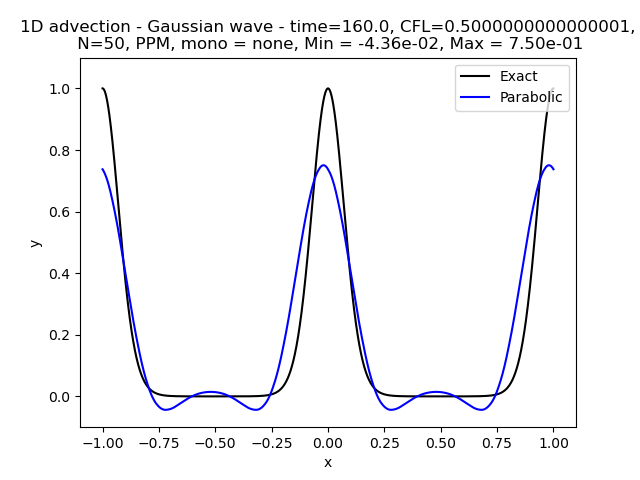
\includegraphics[width=0.45\linewidth]{1d_adv_tc1_ic2_t800_N50_PPM_mononone}
	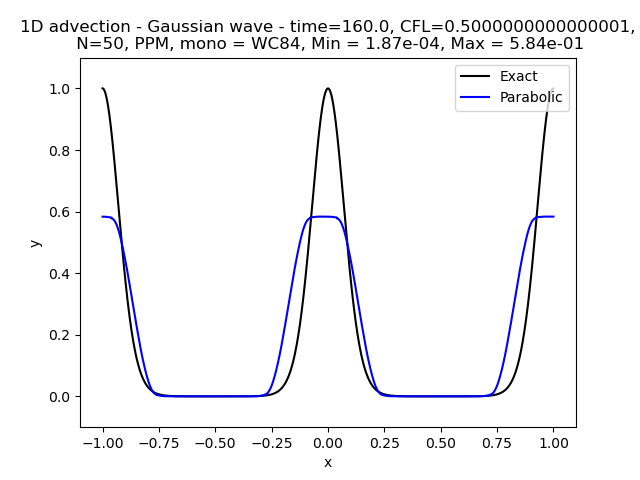
\includegraphics[width=0.45\linewidth]{1d_adv_tc1_ic2_t800_N50_PPM_monoWC84}
	\caption{Gaussian profile after being advected for 1 period without monotonization (left) and
		with monotonization constraint (right).}
	\label{ppm-exp-gaussian}
\end{figure}

\begin{figure}[ht]
	\centering
	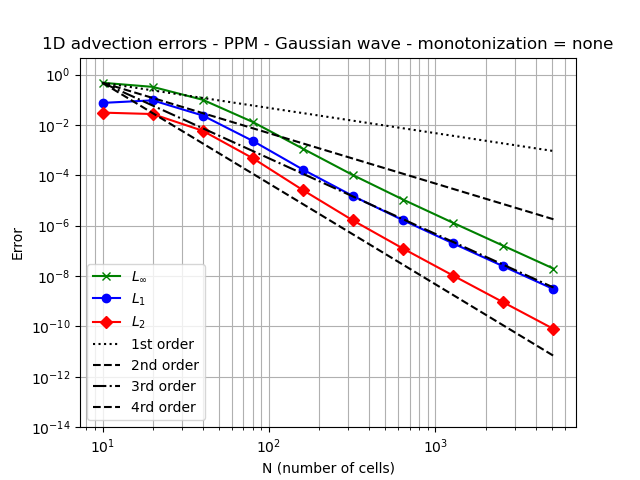
\includegraphics[width=0.45\linewidth]{1d_adv_tc2_PPM_mononone_ic2_parabola_errors}
	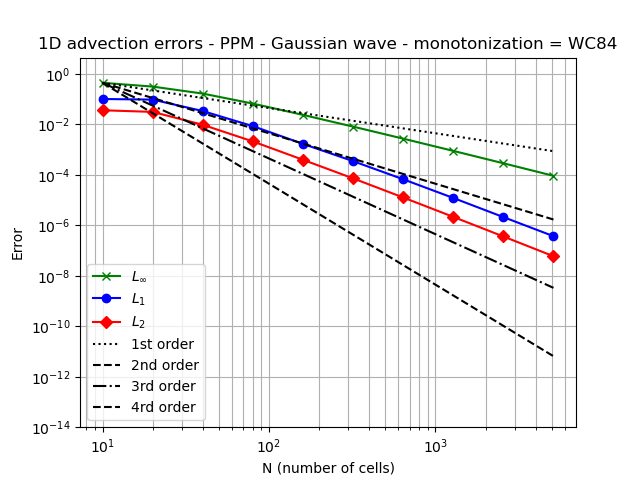
\includegraphics[width=0.45\linewidth]{1d_adv_tc2_PPM_monoWC84_ic2_parabola_errors}
	\caption{Gaussian profile error after being advected for 1 period without monotonization (left) and
	with monotonization constraint (right).}
	\label{ppm-exp-gaussian-errors}
\end{figure}

The first test case consider as initial condition and a constant velocity.
We show the Gaussian profile after one period revolution in Figure \ref{ppm-exp-gaussian}
and in Figure \ref{ppm-exp-gaussian-errors} we depict the error convergence.
We can notice that, PPM reaches the expected third-order and, when we add the monotonization constraint,
the order approaches to one, which is in agreement with the well-known Godunov's theorem \citet{leveque:2002}.
Furthermore, the monotonization constraint removes the dispersion of the method
but adds more numerical diffusion.

\begin{figure}[ht]
	\centering
	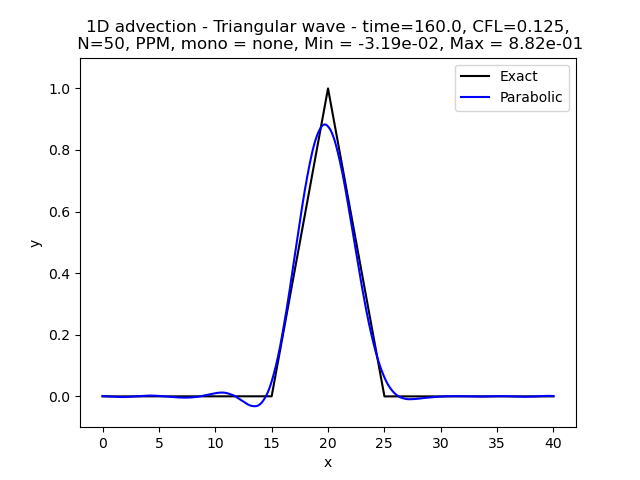
\includegraphics[width=0.4 \linewidth]{1d_adv_tc1_ic3_t800_N50_PPM_mononone}
	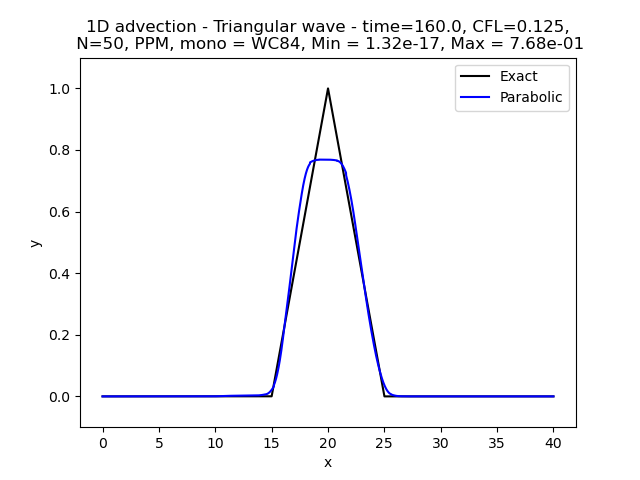
\includegraphics[width=0.4 \linewidth]{1d_adv_tc1_ic3_t800_N50_PPM_monoWC84}
	\caption{Triangular wave after being advected for 1 period without monotonization (left) and
	with monotonization constraint (right).}
	\label{ppm-exp-triangular}
\end{figure}

\begin{figure}[ht]
	\centering
	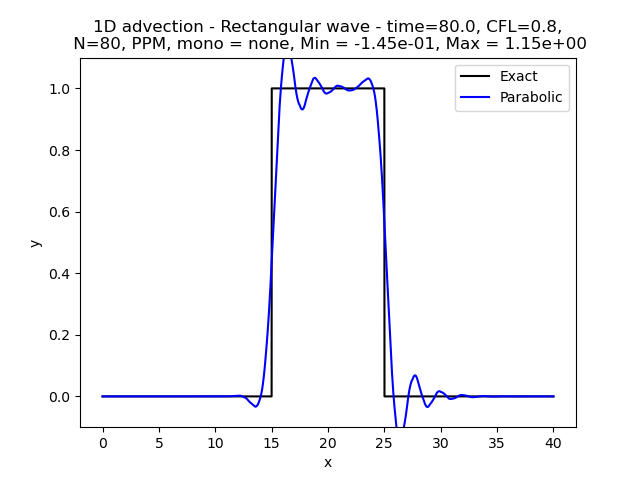
\includegraphics[width=0.4 \linewidth]{1d_adv_tc2_ic4_t100_N80_PPM_mononone}
	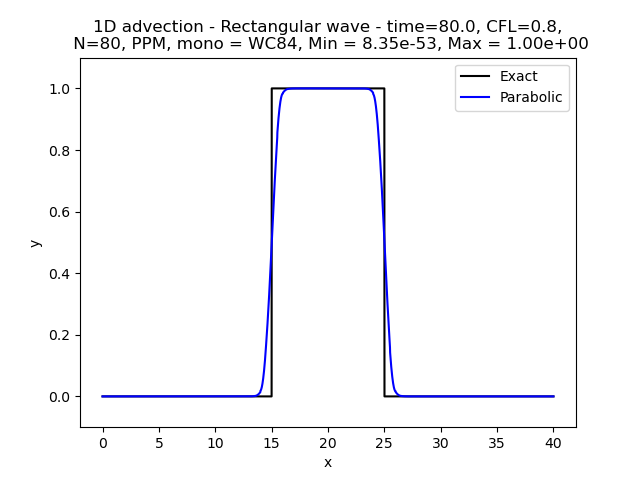
\includegraphics[width=0.4 \linewidth]{1d_adv_tc2_ic4_t100_N80_PPM_monoWC84}
	\caption{Rectangular wave after being advected for 1 period without monotonization (left) and
	with monotonization constraint (right).}
	\label{ppm-exp-rectangular}
\end{figure}

Finally, we show in Figures \ref{ppm-exp-triangular} and \ref{ppm-exp-rectangular}
the results after applying the PPM for the linear advection equation with
constant velocity considering a triangular and a rectangular wave, respectively.
Again, we can notice that the monotonicity constraint reduces greatly the 
dispersion but more diffusion is added, especially in the triangular wave.

